% DPF 09 talk on strangeness in nucleon

\documentclass[10pt]{beamer}
\usepackage{amsmath}
\usefonttheme{professionalfonts} % using non standard fonts for beamer
\usefonttheme{serif} % default family is serif\
\usepackage{mathtools}
%\documentclass[12pt]{beamerthemeSam.sty}
\usepackage{epsf}
%\usepackage{pstricks}
%\usepackage[orientation=portrait,size=A4]{beamerposter}
\geometry{paperwidth=160mm,paperheight=120mm}
%DT favorite definitions
\def\LL{\left\langle}	% left angle bracket
\def\RR{\right\rangle}	% right angle bracket
\def\LP{\left(}		% left parenthesis
\def\RP{\right)}	% right parenthesis
\def\LB{\left\{}	% left curly bracket
\def\RB{\right\}}	% right curly bracket
\def\PAR#1#2{ {{\partial #1}\over{\partial #2}} }
\def\PARTWO#1#2{ {{\partial^2 #1}\over{\partial #2}^2} }
\def\PARTWOMIX#1#2#3{ {{\partial^2 #1}\over{\partial #2 \partial #3}} }

\def\rightpartial{{\overrightarrow\partial}}
\def\leftpartial{{\overleftarrow\partial}}
\def\diffpartial{\buildrel\leftrightarrow\over\partial}

\def\BI{\begin{itemize}}
\def\EI{\end{itemize}}
\def\BE{\begin{displaymath}}
\def\EE{\end{displaymath}}
\def\BEA{\begin{eqnarray*}}
\def\EEA{\end{eqnarray*}}
\def\BNEA{\begin{eqnarray}}
\def\ENEA{\end{eqnarray}}
\def\EL{\nonumber\\}


\newcommand{\map}[1]{\frame{\frametitle{\textbf{Course map}}
\centerline{\includegraphics[height=0.86\paperheight]{../../map/#1.png}}}}
\newcommand{\wmap}[1]{\frame{\frametitle{\textbf{Course map}}
\centerline{\includegraphics[width=0.96\paperwidth]{../../map/#1.png}}}}

\newcommand{\etal}{{\it et al.}}
\newcommand{\gbeta}{6/g^2}
\newcommand{\la}[1]{\label{#1}}
\newcommand{\ie}{{\em i.e.\ }}
\newcommand{\eg}{{\em e.\,g.\ }}
\newcommand{\cf}{cf.\ }
\newcommand{\etc}{etc.\ }
\newcommand{\atantwo}{{\rm atan2}}
\newcommand{\Tr}{{\rm Tr}}
\newcommand{\dt}{\Delta t}
\newcommand{\op}{{\cal O}}
\newcommand{\msbar}{{\overline{\rm MS}}}
\def\chpt{\raise0.4ex\hbox{$\chi$}PT}
\def\schpt{S\raise0.4ex\hbox{$\chi$}PT}
\def\MeV{{\rm Me\!V}}
\def\GeV{{\rm Ge\!V}}

%AB: my color definitions
%\definecolor{mygarnet}{rgb}{0.445,0.184,0.215}
%\definecolor{mygold}{rgb}{0.848,0.848,0.098}
%\definecolor{myg2g}{rgb}{0.647,0.316,0.157}
\definecolor{abtitlecolor}{rgb}{0.0,0.255,0.494}
\definecolor{absecondarycolor}{rgb}{0.0,0.416,0.804}
\definecolor{abprimarycolor}{rgb}{1.0,0.686,0.0}
\definecolor{Red}           {cmyk}{0,1,1,0}
\definecolor{Grey}           {cmyk}{.7,.7,.7,0}
\definecolor{Lg}           {cmyk}{.4,.4,.4,0}
\definecolor{Blue}          {cmyk}{1,1,0,0}
\definecolor{Green}         {cmyk}{1,0,1,0}
\definecolor{Brown}         {cmyk}{0,0.81,1,0.60}
\definecolor{Black}         {cmyk}{0,0,0,1}

\usetheme{Madrid}


%AB: redefinition of beamer colors
%\setbeamercolor{palette tertiary}{fg=white,bg=mygarnet}
%\setbeamercolor{palette secondary}{fg=white,bg=myg2g}
%\setbeamercolor{palette primary}{fg=black,bg=mygold}
\setbeamercolor{title}{fg=abtitlecolor}
\setbeamercolor{frametitle}{fg=abtitlecolor}
\setbeamercolor{palette tertiary}{fg=white,bg=abtitlecolor}
\setbeamercolor{palette secondary}{fg=white,bg=absecondarycolor}
\setbeamercolor{palette primary}{fg=black,bg=abprimarycolor}
\setbeamercolor{structure}{fg=abtitlecolor}

\setbeamerfont{section in toc}{series=\bfseries}

%AB: remove navigation icons
\beamertemplatenavigationsymbolsempty
\title{
  \textbf {Rotational motion}\\
%\centerline{}
%\centering
%\vspace{-0.0in}
%\includegraphics[width=0.3\textwidth]{propvalues_0093.pdf}
%\vspace{-0.3in}\\
%\label{intrograph}
}

\author[W. Freeman] {Physics 211\\Syracuse University, Physics 211 Spring 2016\\Walter Freeman}

\date{\today}

\begin{document}

\frame{\titlepage}

\frame{\frametitle{\textbf{Announcements}}
\BI
\Large
\item{Homework due Friday} 
\item{Office hours today 3:30-5:30}
\item{Review for Exam 3 on Thursday}
\item{Exam 3 next Tuesday}
\EI
}

\frame{\frametitle{\textbf{Exam 3}}
\Large
Topics covered:
\BI
\item{The work-energy theorem}
\item{Potential energy and conservation of energy}
\item{Elasticity and Hooke's law}
\item{Torque and rotational motion}
\EI
You may expect:
\BI
\item{More conceptual problems (no hard math) similar to the multiple choice questions last time}
\item{Problems involving the work-energy theorem in combination with force diagrams or rotation}
\item{Very few problems that require calculator-work}
\EI
}

\frame{\frametitle{\textbf{Exam 3 preparation and end-of-term schedule}}
\large
\BI
\item{Wednesday afternoon: a good time to come to me with grade issues}
\item{Thursday: office hours 1:30-3:30}
\item{Friday: office hours and/or review 10-12 (location TBA) and 1-4 if people aren't at Mayfest}
\item{Saturday: review 4-8 (Clinic/Stolkin)}
\item{Sunday: review 2-5}
\item{Monday: Office hours by appointment; dealing with exam printing}
\item{Tuesday: grading all day}
\item{Wednesday: grading all day, calculating your provisional grades}
\item{Thursday: I hope to have provisional grades available to you after noon}
\item{Friday: review 10-4 (location TBA)}
\item{Saturday: review 2-6 (Physics Clinic/Stolkin)}
\item{Monday: Exam 3 Retake}
\item{Tuesday: GTA's have exams...}
\item{Wednesday: Grading}
\item{Final grades should be done by Friday, May 13}
\EI
}

\frame{\frametitle{\textbf{Exam 3 preparation}}
\Large
\centerline{This is an enormous amount of extra help; use it!}
}

\frame{\frametitle{\textbf{Homework questions}}
\Large
\centerline{Any questions about HW7, HW8, or the practice exam?}
}

\frame{\frametitle{\textbf{Vector torque, the gyroscope, and angular momentum}}



\centerline{(This material will not be treated numerically on your exam, but may appear in conceptual form)}

\vspace{1in}

\large
\centerline{So far we have learned that torque is either CCW (positive) or CW (negative)}
\centerline{... but in 3D, torques can also change the {\it plane of rotation}}
\bigskip
\color{Red}How do we handle situations that don't just change the rate of rotation, but its orientation?
\bigskip
\pause
\bigskip
\centerline{{\color{Blue} ... we need to treat torque and angular momentum as vectors!}}
}

\frame{\frametitle{\textbf{The angular momentum vector}}
\begin{columns}
\column{0.7\textwidth}
\BI
\item{Definition: The angular momentum vector points along the axis of rotation}
\item{... in the direction from which it appears to be going counterclockwise}
\item{... see live demonstration for an example}
\EI
\column{0.3\textwidth}
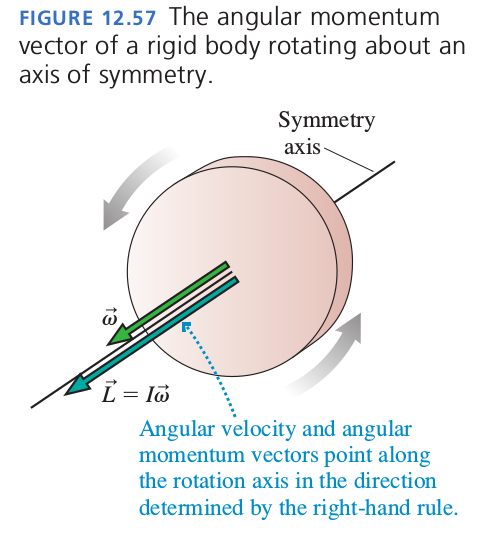
\includegraphics[width=\textwidth]{angular-momentum.png}
\end{columns}
}

\frame{\frametitle{\textbf{The torque vector}}
\large
Torque as a vector has the same magnitude as you've already learned: $$\tau = F_\perp r = F r \sin \theta$$.

Which way does it point?
\normalsize
\Large
\BI
\item{\color{Red}Method 1: $\vec \tau$ points in the direction of the $\vec L$ it creates}
\large
\item{``Torque points along the axle of the wheel pointing toward an observer who sees it as clockwise''}
\Large
\bigskip
\item{\color{Blue}Method 2: $\vec \tau = \vec r \times \vec F$}
\large
\item{...this is a new mathematical idea called the ``cross product''}
\EI
}

\frame{\frametitle{\textbf{The cross product}}
Recall that you already learned about the ``vector dot product'': $\vec A \cdot \vec B = A_\parallel B = A B_\parallel = AB\cos\theta$.

\BI
\item{$\vec A \cdot \vec B$ is a {\color{Red}scalar}}
\EI

\bigskip

The magnitude of the cross product looks similar: $\vec r \times \vec F = F_\perp r = F r_\perp = Fr\sin\theta$. 
(Look familiar?)
 
\BI
\item{... but $\vec r \times \vec F$ is a {\color{Red}vector}}
\pause
\item{Which way does it point? Use the ``right hand rule'':}
\centerline{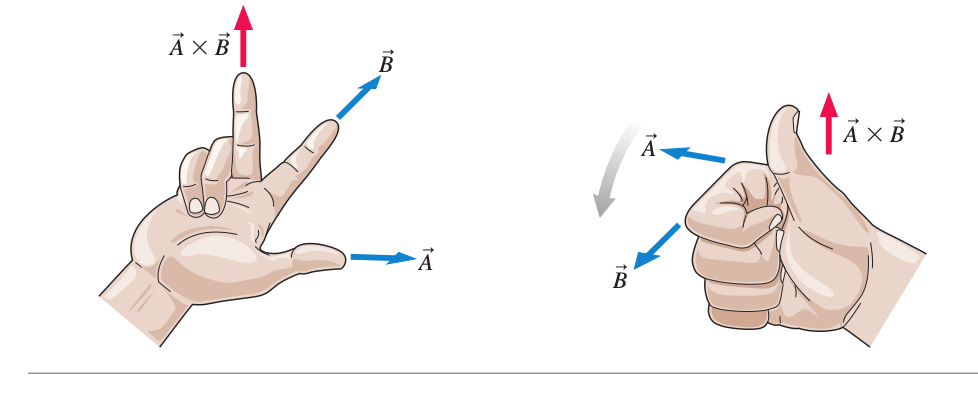
\includegraphics[width=0.5\textwidth]{rhr.png}}
\EI

\BI
\item{Thumb goes in the direction of $\vec r$, pointer goes in the direction of $\vec F$, middle finger shows you $\vec \tau$}
\item{Point fingers in the direction of $\vec r$, curl them in the direction of $\vec F$; thumb tells you the direction of $\vec \tau$}
\EI

This gets you the same result for the direction of the torque.

(Knowing about the cross product and the dot product will be {\bf very important} in Physics 2!)}

\frame{\frametitle{\textbf{The angular momentum vector, again}}

We can also say that {\color{Red} $\vec L = m \vec r \times \vec v$}

(Note that this matches our formula from before: $L = m v_T r$)

Here the right-hand rule tells us that $\vec L$ points out of the board.

This matches our other definition: ``$\vec L$ points toward an observer that sees rotation as counterclockwise.``

\centerline{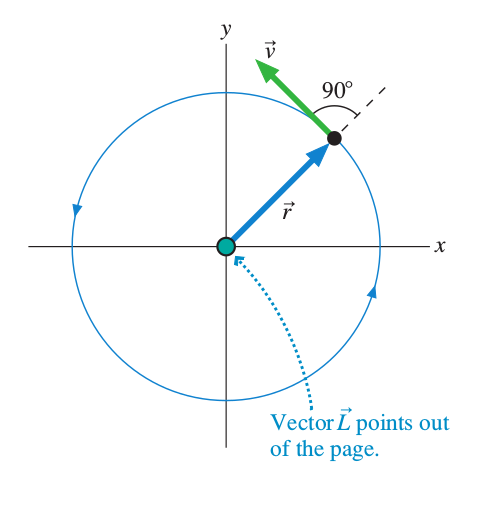
\includegraphics[width=0.3\textwidth]{angular-momentum-2.png}}

\pause

One detail: $\vec \omega$ only points in the same direction as $\vec L$ if the object is rotating ``mostly'' about an axis of symmetry.\\
Otherwise, $\omega$ behaves chaotically; the object tumbles.
}


\frame{\frametitle{\textbf{The magic wheel, explained}}
\large

What direction does $\vec L$ point?

\pause

\BI
\item{$\vec L$ points (as I'm showing it here) along the axle, away from the string}
\EI

\bigskip

What direction does $\vec \tau$ point?

\BI
\item{$\vec \tau$ points horizontally, ``around'' the circle}
\EI

\pause

\centerline{Recall that $\vec \tau$ is the rate of change of $\vec L$, so gravity doesn't make it fall -- just ``rotates'' the axis of rotation around!}
\centerline{This works the same way as an ordinary top}
}


\frame{\frametitle{\textbf{The gyroscope}}
\large

An object that is spinning rapidly has a great deal of angular momentum.

Since its angular momentum vector is so ``long'', it resists changes in its direction.

We can do two things with this: 

\BI
\item{Since its axis stays fixed, we can use it to determine how {\it we've} rotated}
\item{Since it has so much $\vec L$, we can apply torques to it without affecting its axis of rotation much.}
\BI
\item{By Newton's third law, these forces also exert a torque on something else}
\item{This can be used to orient a free-floating object, like the Hubble Space Telescope}
\EI
\EI
}

\frame{\frametitle{\textbf{... boom!}}
\Large

\centerline{How fast can we propel a ping-pong ball using nothing at all?}
}



\end{document}


